% !TeX document-id = {2385fae9-28e6-4c73-97cb-b86e8670f6e7}
\documentclass[titlepage]{article}
\usepackage[upright]{fourier}
\usepackage[utf8]{inputenc}
\usepackage[french]{babel}
\usepackage[margin=1in]{geometry}
\usepackage[T1]{fontenc}

\usepackage[colorlinks=true,linkcolor=teal]{hyperref}
\usepackage{amssymb,amsmath,minted,float,graphicx,textcomp,systeme,listings,physics,mathtools,ifthen,esvect,hyperref,fancyhdr,lastpage,marginnote,chngcntr,fancyvrb,subcaption}
\usepackage{stmaryrd}
\usepackage{minted}
\DeclareMathOperator{\e}{e}
\def\mathbi#1{\textbf{\em #1}}

\setlength\parindent{0pt}

%%%%%%%%%%%% PARAMETRES
\newcommand{\UE}{Stage}
\newcommand{\type}{Résultats}%TD-TP-COURS
\newcommand{\nb}{0}%nb 
\newcommand{\sbt}{Reconstruction dynamique d'images radioastronomiques}%soustitre
\author{Gabriel ROBERT-DAUTUN}
\date{2022}

% mise en page (header, compteur, fancy)
\pagestyle{fancy}
\lhead{\UE\, - \type\ifthenelse{\nb > 0}{\nb}{}}
\rfoot{\thepage /\pageref{LastPage}}
\lfoot{}
\cfoot{}
\renewcommand{\footrulewidth}{0.4pt}

%reset compteur section par partie
\counterwithin*{section}{part}

% permet notes + simples en marge à gauche (ig compteur de question)
\reversemarginpar
\newcommand{\mgn}[1]{\marginnote{#1}}

%sinon warning mdr
\setlength{\headheight}{13.07225pt}

%compteur questions
\newcounter{question}
\setcounter{question}{1}
\newcounter{subq}
\setcounter{subq}{1}

\newcommand{\rsubq}{\setcounter{subq}{1}}
\newcommand{\question}{\mgn{\thequestion .}\stepcounter{question}\rsubq}
\newcommand{\rstq}{\setcounter{question}{1}\rsubq}
\newcommand{\skipq}[1]{\addtocounter{question}{#1}\rsubq}
\newcommand{\subq}{\noindent\alph{subq})\stepcounter{subq}} %a modifier pour mettre dans le margin

\newcommand{\C}{\mathcal{C}}
\newcommand{\Ht}{\widetilde{H}}
\newcommand{\Hc}{\C\odot\Ht}
\newcommand{\B}{\mathcal{B}}
\newcommand{\Hb}{\B\odot\Ht}
\newcommand{\hinv}[1]{#1^{\circ-1}}

\title{%
	\UE\, - \type\ifthenelse{\nb > 0}{\nb}{} \\
	\large \sbt}

\begin{document}
	
	\begin{figure}
		\centering
		
\includegraphics[width=0.7\linewidth]{logo.PNG}
		\label{fig:logo}
	\end{figure}
	\maketitle
	
	\newpage
	\tableofcontents
	
	\newpage
	\section{Notations}
	\subsection{Produit de Hadamard}
	
	On introduit la notation $\odot$ associée au produit de Hadamard, qui effectue la multiplication élément à élément de deux matrices de même taille :
	$$
	\forall (A,B)\in\left(\mathbb{C}^{m\times n}\right)^2, \quad A\odot B\in\mathbb{C}^{m\times n} \quad\text{et}\quad \forall (i,j)\in\llbracket1;m\rrbracket\times\llbracket1;n\rrbracket,\, (A\odot B)_{i,j} = A_{i,j}\times B_{i,j}
	$$
	
	On introduit également l'inverse de Hadamard, qui inverse élément par élément une matrice
	$$
		\forall A \in \left(\mathbb{C}\backslash\{0\}\right)^{m\times n},\quad \hinv{A}\in\left(\mathbb{C}\backslash\{0\}\right)^{m\times n} \quad\text{et}\quad \forall (i,j)\in\llbracket1;m\rrbracket\times\llbracket1;n\rrbracket,\, \left(\hinv{A}\right)_{i,j} = \left(A_{i,j}\right)^{-1}
	$$ 
	
	\newpage
	\section{Influence individuelle de l'erreur sur les matrices}
	\subsection{Erreur sur l'image de départ}
	On introduit une erreur gaussienne sur l'image $X_0$. On observe que le fonctionnement du Kalman est bien celui attendu dans ce cas là : l'erreur dans l'image se réduit petit a petit.
	
	\begin{figure}[H]
		\centering
		\includegraphics[width=0.9\linewidth]{Perfs/Illustration.JPG}
		\caption{En haut : images réelles utilisées pour générer les données. En bas : images reconstruites. Titres : PSNR}
	\end{figure}

	On utilise une transformation de rotation de l'image de 90°. On remarque grâce au PSNR que les images reconstruites s'approchent des images réelles, mais pas parfaitement car le filtre prend en compte l'historique. Une erreur dans une image va donc se diffuser aux images suivantes (précédentes si backwards). On observe la convergence de reconstruction :
	
	\begin{figure}[H]
		\centering
		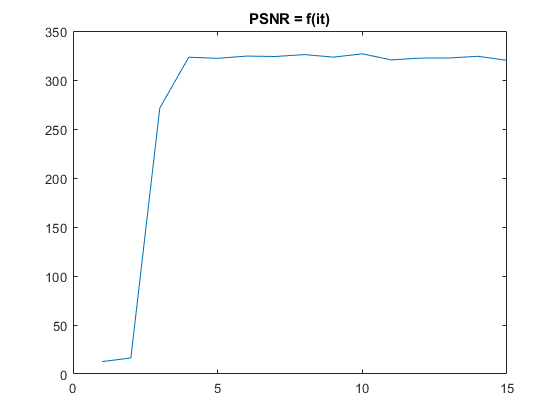
\includegraphics[width=0.9\linewidth]{Perfs/conv02.png}
		\caption{Evolution psnr en fonction du nombre d'itérations}
	\end{figure}

	On converge en 4 itérations au plus a chaque essai : les erreurs gaussienne d'amplitude 0.2 se diffusent sur 4 itérations environ.
	Vérifié pour des amplitude de 0.1 a 1. Pour des amplitudes plus grandes (5 donc SNR=0.1) parfois 5 itérations sont nécessaires.
	
	\subsection{Erreur sur les matrices de covariance}
	
	Les matrices $\{P_k\}$ et $\{Q_k\}$ servent à calculer le gain de Kalman et donc sélectionner quelle proportion mesure/prédiction choisir pour estimer l'image. Si on introduit une erreur \emph{uniquement} sur une de ces matrices, l'image prédite et l'image mesurée seront les mêmes (car on y a pas introduit d'erreur) et donc une erreur sur la proportion n'aura aucun effet.\\
	Une erreur sur ces matrices n'introduit donc pas d'erreur sur la reconstruction de manière directe. Elle peut néanmoins diffuser une erreur déjà présente.
	
	\subsection{Erreur sur le modèle d'évolution}
	
	On suppose une erreur sur le modèle d'évolution \emph{dans le filtre de Kalman}, afin de simuler un modèle théorique imprécis. On construit les données simulées avec un modèle sans erreur.\\
	\begin{minted}{matlab}
poids = 0.2;
A = A + poids*randn(size(A));
	\end{minted}
	
	On introduit une erreur gaussienne
	
	\subsection{Erreur sur le masque UV}
	
	On cherche à caractériser l'erreur sur la matrice du plan UV $H$. Une manière naïve de faire le calcul serait d'ajouter une erreur gaussienne comme sur la matrice $A$, mais en faisant cela on obtient un modèle très instable et peu réaliste. Effectivement, les termes de cette matrices étant :
	$$
		H_{j,q} = \exp(-j\frac{2\pi}{\lambda}\Delta z_j\dotproduct\mathbf{I}_q)
	$$
	L'erreur sur cette matrice pouvant provenir de différentes sources : mauvaise mesure des distances entre les antennes, mauvais alignement des antennes donc erreur sur les directions, le modèle d'erreur est :
	$$
		H_{j,q}^{err} =  \exp(-i\frac{2\pi}{\lambda}(\Delta z_j\dotproduct\mathbf{I}_q + \varepsilon)) =  \exp(-i\frac{2\pi}{\lambda}\Delta z_j\dotproduct\mathbf{I}_q)\exp(-i\frac{2\pi}{\lambda}\varepsilon\dotproduct\mathbf{I}_q)
	$$
	
	Soit une rotation du complexe associé a chaque direction. \\
	
	On implémente donc l'erreur de la manière suivante pour quantifier l'erreur acceptable sur les positions des antennes :
	
	\begin{minted}{matlab}
poids = 1e-2;
z_err = z+ randn(size(z))*poids;
H_err = matF(J,Pix,z_err,lambda,I);
	\end{minted}

	On peut ensuite mesurer l'évolution du PSNR dans le temps, pour différents écarts possibles :
	
%	\begin{figure}[H]
%		\centering
%		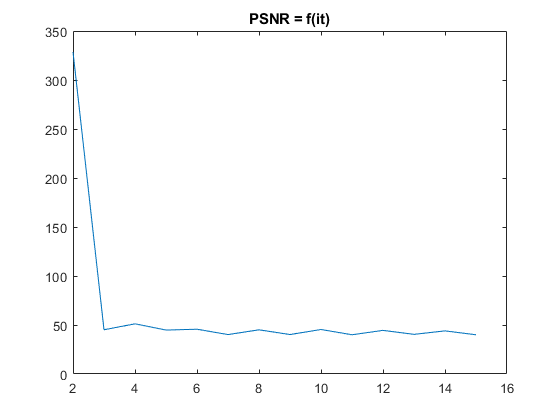
\includegraphics[width=0.7\linewidth]{Perfs/H5e-3}
%		\caption{Evolution du PSNR pour $<\varepsilon^2>=5$mm}
%		\label{fig:h5e-3}
%	\end{figure}
%	
%	\begin{figure}[H]
%		\centering
%		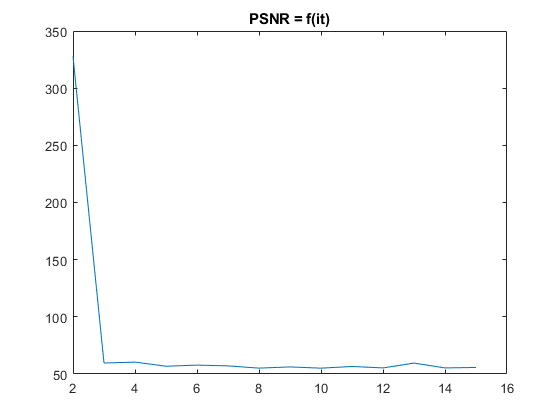
\includegraphics[width=0.7\linewidth]{Perfs/He-3_1}
%		\caption{Evolution du PSNR pour $<\varepsilon^2>=1$mm}
%		\label{fig:he-3}
%	\end{figure}
%	
%	\begin{figure}[H]
%		\centering
%		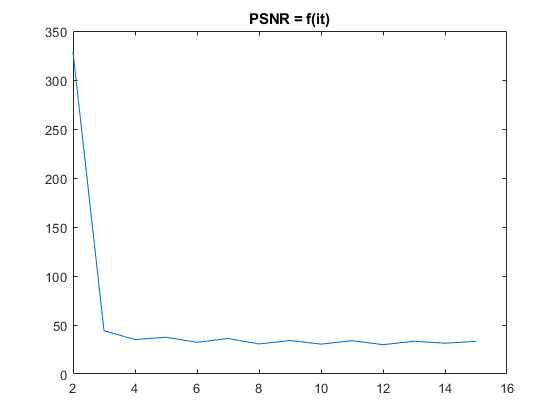
\includegraphics[width=0.7\linewidth]{Perfs/He-2}
%		\caption{Evolution du PSNR pour $<\varepsilon^2>=1$cm}
%		\label{fig:he-2}
%	\end{figure}
	
	\begin{figure}[H]
		\centering
		\begin{subfigure}{.5\textwidth}
			\centering
			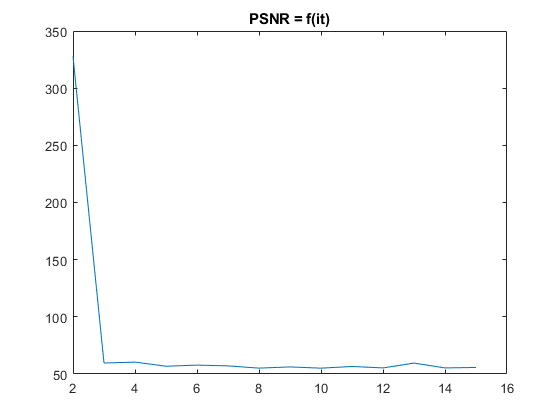
\includegraphics[width=0.9\linewidth]{Perfs/He-3_1}
			\caption{Evolution du PSNR pour $<\varepsilon^2>=1$mm}
			\label{fig:he-3}
		\end{subfigure}%
		\begin{subfigure}{.5\textwidth}
			\centering
			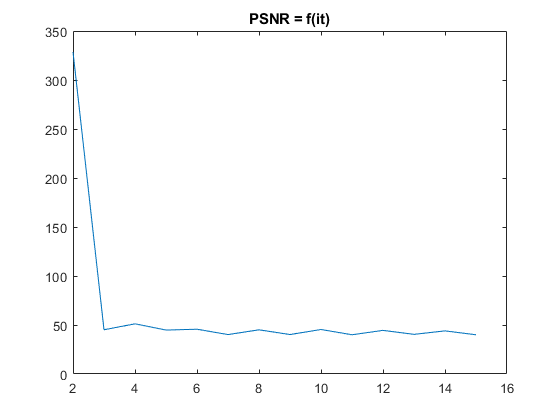
\includegraphics[width=0.9\linewidth]{Perfs/H5e-3}
			\caption{Evolution du PSNR pour $<\varepsilon^2>=5$mm}
			\label{fig:h5e-3}
		\end{subfigure}
		\begin{subfigure}{.5\textwidth}
			\centering
			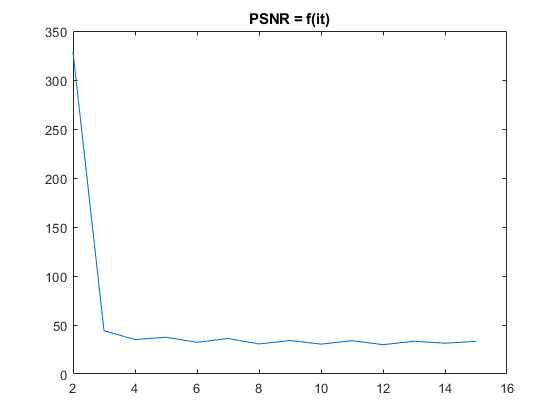
\includegraphics[width=0.9\linewidth]{Perfs/He-2}
			\caption{Evolution du PSNR pour $<\varepsilon^2>=1$cm}
			\label{fig:he-2}
		\end{subfigure}
		\caption{Mesure du psnr pour différentes erreurs sur la position}
	\end{figure}

	Les mesures obtenues ont \emph{généralement} cette forme : on obtient parfois des évolutions sans le pic au début, mais la mesure va toujours converger vers une valeur identique tant que $<\varepsilon^2>$ reste constant, en oscillant autour de cette valeur. On peut donc tracer l'évolution de l'erreur de reconstruction en fonction de $<\varepsilon^2>$ :
	
	\begin{figure}[H]
		\centering
		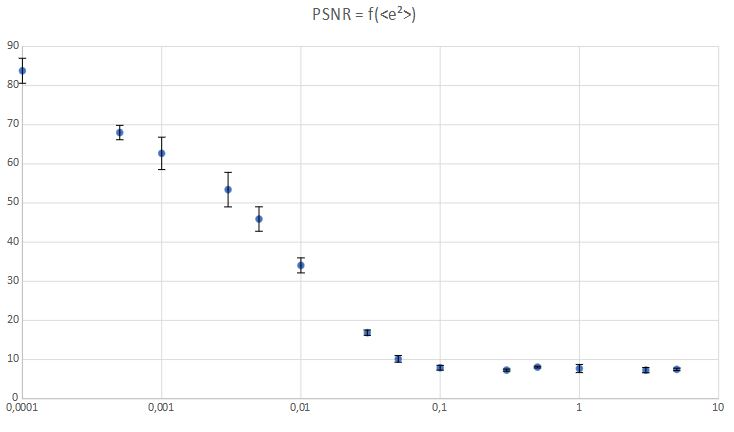
\includegraphics[width=0.7\linewidth]{Perfs/perf_errF}
		\caption{Qualité de reconstruction en fonction de l'erreur}
	\end{figure}

	\subsubsection{Calculs théoriques}
	
	On considère la matrice $\widetilde{H}$ construite avec une erreur de mesure sur la position des antennes, c'est à dire 
	$$
		\forall j \in \llbracket1;J^2\rrbracket,\:\: \widetilde{\Delta} z_j = \Delta z_j + \boldsymbol{\varepsilon}_j
	$$
	On suppose l'erreur $\boldsymbol{\varepsilon}$ suivant une loi normale.\\
	Les termes de la matrice $\widetilde{H}$ deviennent :
	$$
		\widetilde{H}_{j,q} = \exp(-i\frac{2\pi}{\lambda}\widetilde{\Delta}z_j\dotproduct\mathbf{I}_q) = H_{j,q}\times\exp(-i\frac{2\pi}{\lambda}\boldsymbol{\varepsilon}_j\dotproduct\mathbf{I}_q)
	$$
	

	On peut donc établir une matrice de correction $\mathcal{C}$ telle que :
	$$
		H = \mathcal{C}\odot\widetilde{H}
	$$
	\newpage
	
	On peut vérifier que l'expression de $K$ reste inchangée : on exprime $P_{k|k}$ :
	\begin{align*}
		P_{k|k} &= E\left[\left(\widehat{x}_{k|k} - x_k\right)\left(\widehat{x}_{k|k} - x_k\right)^H\right] \\
		&= E\left[\left(\widehat{x}_{k|k-1} + K(y_k - H\widehat{x}_{k|k-1}) - x_k\right)\left(\widehat{x}_{k|k-1} + K(y_k - H\widehat{x}_{k|k-1}) - x_k\right)^H\right] \\
		&= E\left[\left(\widehat{x}_{k|k-1} - K(\C\odot\widetilde{H})\widehat{x}_{k|k-1} + Ky_k - x_k\right)\left(\widehat{x}_{k|k-1} - K(\C\odot\widetilde{H})\widehat{x}_{k|k-1} + Ky_k - x_k\right)^H\right] \\
		&= E\left[\left((\widehat{x}_{k|k-1}-x_k) -K(\C\odot\widetilde{H})(\widehat{x}_{k|k-1}-x_k) + K(y_k - (\C\odot\widetilde{H})x_k)\right)\left((\widehat{x}_{k|k-1}-x_k) -K(\C\odot\widetilde{H})(\widehat{x}_{k|k-1}-x_k) + K(y_k - (\C\odot\widetilde{H})x_k)\right)^H\right]
	\end{align*}
	
	On peut faire apparaître les erreurs de mesure $\varepsilon_{mes}$ et de prédiction $\varepsilon_{pred}$ :
	\begin{align*}
		\varepsilon_{mes} &= y_k - (\C\odot\widetilde{H})x_k \\
		\varepsilon_{pred} &= \widehat{x}_{k|k-1} - x_k
	\end{align*}

	Ces erreurs sont décorrelées, donc les termes correspondant seront nuls :
	$$
		E\left[\varepsilon_{mes}\varepsilon_{pred}^H\right] = 0
	$$
	
	En rappelant de plus :
	\begin{align*}
		P_{k|k-1} &= E\left[\varepsilon_{pred}\varepsilon_{pred}^H\right] \\
		R &=  E\left[\varepsilon_{mes}\varepsilon_{mes}^H\right]
	\end{align*}

	Erreurs aux indices k, on peut développer la formule de $P_{k|k}$
	
	\begin{align*}
		P_{k|k} &= P_{k|k-1} + K\left(\C\odot \widetilde{H}\right)P_{k|k-1}\left(\Hc\right)^H - P_{k|k-1}\left(K\Hc\right)^H - K\left(\Hc\right)P_{k|k-1} + KRK^H
	\end{align*}
	
	Cette forme est bien minimisée par 
	\begin{equation}
		K_k^c = P_{k|k-1}\left(\Hc\right)^H\left(\left(\Hc\right)P_{k|k-1}\left(\Hc\right)^H + R\right)^{-1}
	\end{equation}
	Forme similaire au gain $K$ calculé sans correction :
	\begin{equation}
		K_k = P_{k|k-1}\Ht^H\left(\Ht P_{k|k-1}\Ht^H + R\right)^{-1}
	\end{equation}

	Par la suite, on omettra les dépendances en $k$ en supposant $P=P_{k|k-1}$ et $K = K_k$.
	
	On pose l'erreur sur le gain :
	\begin{equation}
		\varepsilon_K = K^c - K
	\end{equation}

	Ainsi que l'erreur d'estimation induite par l'erreur de masque :
	\begin{equation}
		\varepsilon_{\widehat{x}} = \widehat{x}_{k|k} - \widehat{x}_{k|k}^c
	\end{equation}
	
	On omettra de la même façon la dépendance en $k$. En développant :
	\begin{align*}
		\varepsilon_{\widehat{x}} &= \left[\widehat{x}_{k|k-1} + K(y_k-\Ht\widehat{x}_{k|k-1})\right] - \left[\widehat{x}_{k|k-1} + K^c\left(y_k - \left(\Hc\right)\widehat{x}_{k|k-1}\right)\right] \\
		&= \left(K-K^c\right)y_k - \left(K\Ht - K^c(\Hc)\right)\widehat{x}_{k|k-1} \\
		&= \varepsilon_K\left[y_k - \left(\Hc\right)\widehat{x}_{k|k-1}\right] + K\left(\mathbb{1}-\C\right)\odot\Ht\widehat{x}_{k|k-1}
	\end{align*}

	Où $\mathbb{1}$ désigne l'élément neutre du produit de Hadamard, la matrice dont tous les termes valent 1.\\	
	Donc :
	\begin{equation}
		\varepsilon_{\widehat{x}} = \varepsilon_K\varepsilon_{mes} + K\left(\mathbb{1} - \mathcal{C}\right)\odot\Ht\widehat{x}_{k|k-1}
	\end{equation}

	Sous l'hypothèse de l'introduction d'erreur uniquement sur $H$, la matrice $\C\odot\Ht$ est la matrice corrigée et on obtient :
	$$
		y_k = \Hc x_k \implies \varepsilon_{mes} = 0
	$$
	D'où :
	\begin{equation}
		\varepsilon_{\widehat{x}} = K \left(\mathbb{1} - \C\right)\odot\Ht\widehat{x}_{k|k-1}
	\end{equation}

	On peut de même évaluer le différentiel sur les covariances :
	\begin{equation}
		\Delta P_{k|k} = P_{k|k} - P_{k|k}^c = \left(K^c\left(\Hc\right) - K\Ht\right)P_{k|k-1}
	\end{equation}

	De plus, si on suppose une erreur de gain sur les antennes, on peut poser les termes :
	$$
		\Ht_{j,q} = (1+\varepsilon_q)H_{j,q}
	$$
	
	Où $\varepsilon_q$ suit une loi normale, et désigne une erreur sur le gain de l'antenne $q$.\\
	On peut de même établir une matrice de correction $\B$ telle que :
	\begin{equation}
		H = \Hb
	\end{equation}

	Les erreurs et gain auront alors la même forme
	\begin{subequations}
		\begin{equation}
			K_k^b = P\left(\Hb\right)^H\left(\left(\Hb\right)P\left(\Hb\right)^H + R\right)^{-1}
		\end{equation}
		\begin{equation}
			\varepsilon_{\widehat{x}} = K\left(\mathbb{1} - \B\right)\odot\Ht\widehat{x}_{k|k-1}
		\end{equation}
		\begin{equation}
			\Delta P_{k|k} = \left(K^b\left(\Hb\right) - K\Ht\right)P_{k|k-1}
		\end{equation}
	\end{subequations}
	
	\subsubsection{Essais expérimentaux}
	
	On effectue des essais en introduisant une erreur sur la matrice exacte. Plutôt que d'avoir une matrice erronée $\Ht$ connue on aura $H$ exacte connue et :
	$$
		\Ht = \mathcal{E}\odot H
	$$
	où $\mathcal{E} = \hinv{\C}$ ou $\mathcal{E} = \hinv{\B}$ en fonction de l'erreur que l'on souhaite introduire.
	
	\paragraph{Erreur de position}
	On suppose tout d'abord que l'on ne connaît pas exactement la position des antennes du réseau. On introduit sur $H$ une matrice de petites rotations définie par la matrice $\mathcal{R} = \hinv{\B}$ plus tôt. \\
	Pour cela, on génère $J^2$ vecteurs $\{\boldsymbol{\varepsilon}_j\}$ et on génère $\mathcal{R}$. 
\end{document}


\begin{figure}[H]
	\centering
	\includegraphics[width=0.7\linewidth]{}
	\caption{}
\end{figure}

\begin{figure}[H]
	\centering
	\begin{subfigure}{.5\textwidth}
		\centering
		\includegraphics[width=.9\linewidth]{image1}
		\caption{}
	\end{subfigure}%
	\begin{subfigure}{.5\textwidth}
		\centering
		\includegraphics[width=.9\linewidth]{image2}
		\caption{}
	\end{subfigure}
	\caption{}
\end{figure}

